\section{Ejercicio 6}

Este punto busca mostrar las diferencias entre \emph{Round-Robin} y \emph{FCFS}.
Para ello, se ejecutó el mismo lote de tareas del ejercicio anterior utilizando
\texttt{SchedFCFS} como scheduler. La cantidad de núcleos se fijó en 1 y el
costo de cambio de contexto en 2.

\begin{figure}[H]
	\begin{center}
		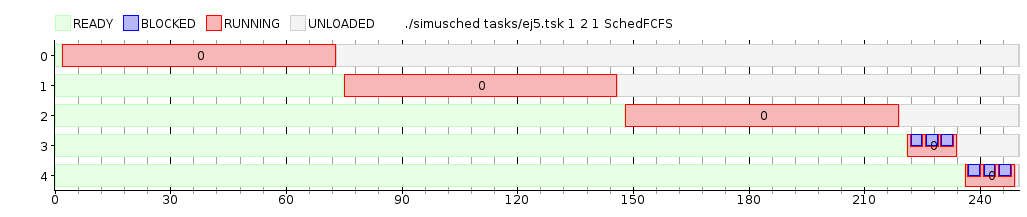
\includegraphics[width=1\columnwidth]{imagenes/ej6.png}
		\caption{\texttt{SchedFCFS} corriendo el lote de tareas del Ejercicio \ref{sec:ej5}}
	\end{center}
\end{figure}

Habiendo graficado el resultado de correr estas tareas con \texttt{SchedFCFS}
uno ya podría llegar a realizar algunas observaciones, pero con el objetivo de
tener más información a la hora de comparar, se calculó la
\emph{latencia}, \emph{waiting-time} y \emph{turnaround} promedio. Los valores
obtenidos se muestran a continuación.

\begin{figure}[H]
	\begin{center}
		\begin{tabular}{|r|c|c|c|c|}
			\hline
			\textbf{Scheduler} & \textbf{Quantum} & \textbf{Latencia} & \textbf{Waiting-time} & \textbf{Turnaround} \\ \hline
			\texttt{SchedRR} & 2 & 9,8 & 250,4 & 298,2 \\ \cline{2-5}
			& 10 & 24,2 & 188 & 235,8 \\ \cline{2-5}
			& 30 & 60,2 & 191,6 & 239,4 \\ \hline
			\texttt{SchedFCFS} & N/A & 136,4 & 136,4 & 184,2 \\ \hline
		\end{tabular}
		\caption{Tiempos promedio en función del scheduler utilizado}
	\end{center}
\end{figure}

Lo primero que llama la atención es la \emph{latencia}, ya que supera de forma
significativa la de las pruebas realizadas con \texttt{SchedRR}. Esto es fácil
de ver dado que cada tarea se corre de principio a fin, antes de cederle el
control a la siguiente. Claramente esta política no sería eficiente a la hora de
querer un sistema con procesos interactivos, ya que el tiempo de respuesta sería
enorme, dando al usuario la sensación de que el mismo dejó de funcionar por
completo.

Por otra parte, el \emph{waiting-time} tanto como el \emph{turnaround} dieron
valores más bajos. Esto se puede justificar con el hecho de que cualquier
implementación de \emph{Round-Robin} contará con el overhead de realizar cambios
de contextos sumado a que cada tarea tiene que esperar a que se de toda la
vuelta para ser asignada de nuevo.

Ahora, al analizarse con más cuidado es posible cuantificar estas diferencias para
poder pesarlas mejor en la balanza. Tomando el resultado de \texttt{SchedRR} con
quantum \textbf{10} y comparándolo contra el de \texttt{SchedFCFS} se tienen los
siguientes porcentajes asociados al último:

\begin{itemize}
	\item 463.6\% más de \emph{latencia}
	\item 37.8\% menos de \emph{waiting-time}
	\item 28\% menos de \emph{turnaround}
\end{itemize}

De aquí se puede apreciar cómo la mejoría en \emph{waiting-time} y
\emph{turnaround} es a cuestas de un gran deterioro en lo que es
\emph{latencia}.

Es por esto que se concluye que \emph{FCFS} tiene sentido cuando no interesa el
tiempo de respuesta y uno está dispuesto a sacrificar esa característica con tal
de obtener una mejoría en otros criterios como lo son el \emph{waiting-time} y
\emph{turnaround}.
